% Chapter 1

\chapter{Project Design} % Main chapter title

\label{Chapter3} % For referencing the chapter elsewhere, use \ref{Chapter1}

\lhead{Chapter 3. \emph{Project Design}} % This is for the header on each page - perhaps a shortened title

%----------------------------------------------------------------------------------------

\section{Methodology}
The methodology adopted for designing the "Track My Shop" web application is an iterative process. The methodology encompasses various stages from project initiation to implementation, ensuring an organized and systematic approach as each stage is mentioned below:

\begin{figure}[h]
	\centering
	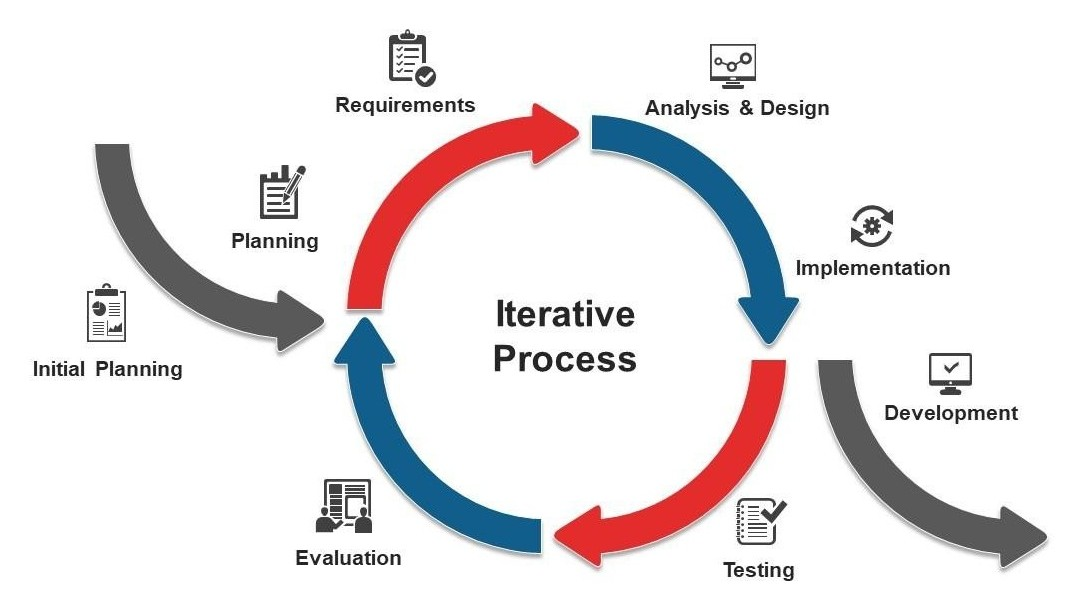
\includegraphics[width=15cm]{iterative_process_model}
	\caption{Iterative Process Model}
\end{figure}

\subsection{Initial Planning}

In this initial planning stage, the project goals and initial requirements are outlined. Key activities include:

\textbf{Defining Project Goals}: Setting the overall goals and vision for the "Track My Shop" application.

\textbf{Preliminary Requirement Analysis}:
Performing an initial analysis of high-level requirements and constraints.

\subsection{Planning}

The planning stage involves planning the upcoming iteration and setting specific goals for it. Key activities include:

\textbf{Setting Iteration Goals}:
Defining the objectives and outcomes for the current iteration.

\textbf{Identifying Resources}:
Allocating the necessary resources, including manpower, technology, and tools, for the iteration.

\subsection{Requirements Analysis and Design}

In this stage, detailed requirements are gathered and analyzed, and the system's design is conceptualized. Key activities include:

\textbf{Requirements Refinement}:
Analyzing and refining requirements based on feedback from previous iterations and stakeholders.

\textbf{System Design}:
Conceptualizing the system's design and architecture based on the refined requirements.

\subsection{Implementation and Development}

The implementation stage involves writing code and developing the iteration. Key activities include:

\textbf{Coding and Development}:
Writing the code based on the design and architecture defined in the previous stage.

\textbf{Integration}:
Integrating the developed components and modules into a cohesive iteration.

\subsection{Testing}

The testing stage involves validating the functionality and performance of the developed iteration. Key activities include:

\textbf{Functional Testing}:
Ensuring that the iteration meets the specified functional requirements.

\textbf{User Acceptance Testing (UAT)}:
Engaging users to validate the iteration against their expectations and requirements.

\subsection{Evaluation}

The evaluation stage involves assessing the outcomes of the iteration. Key activities include:

\textbf{Evaluation of Goals}:
Evaluating whether the iteration goals were achieved and identifying areas for improvement.

\subsection{Summary}

The iterative process model is adopted in the development of the "Track My Shop" application, allowing for incremental development, feedback incorporation, and continuous improvement. Each iteration adds new features, refines existing functionalities, and incorporates feedback for an improved and user-centric product.






\section{Architecture Overview}


\begin{figure}[h]
	\subsection{Entity Relationship Diagram (ERD) }
	\centering
	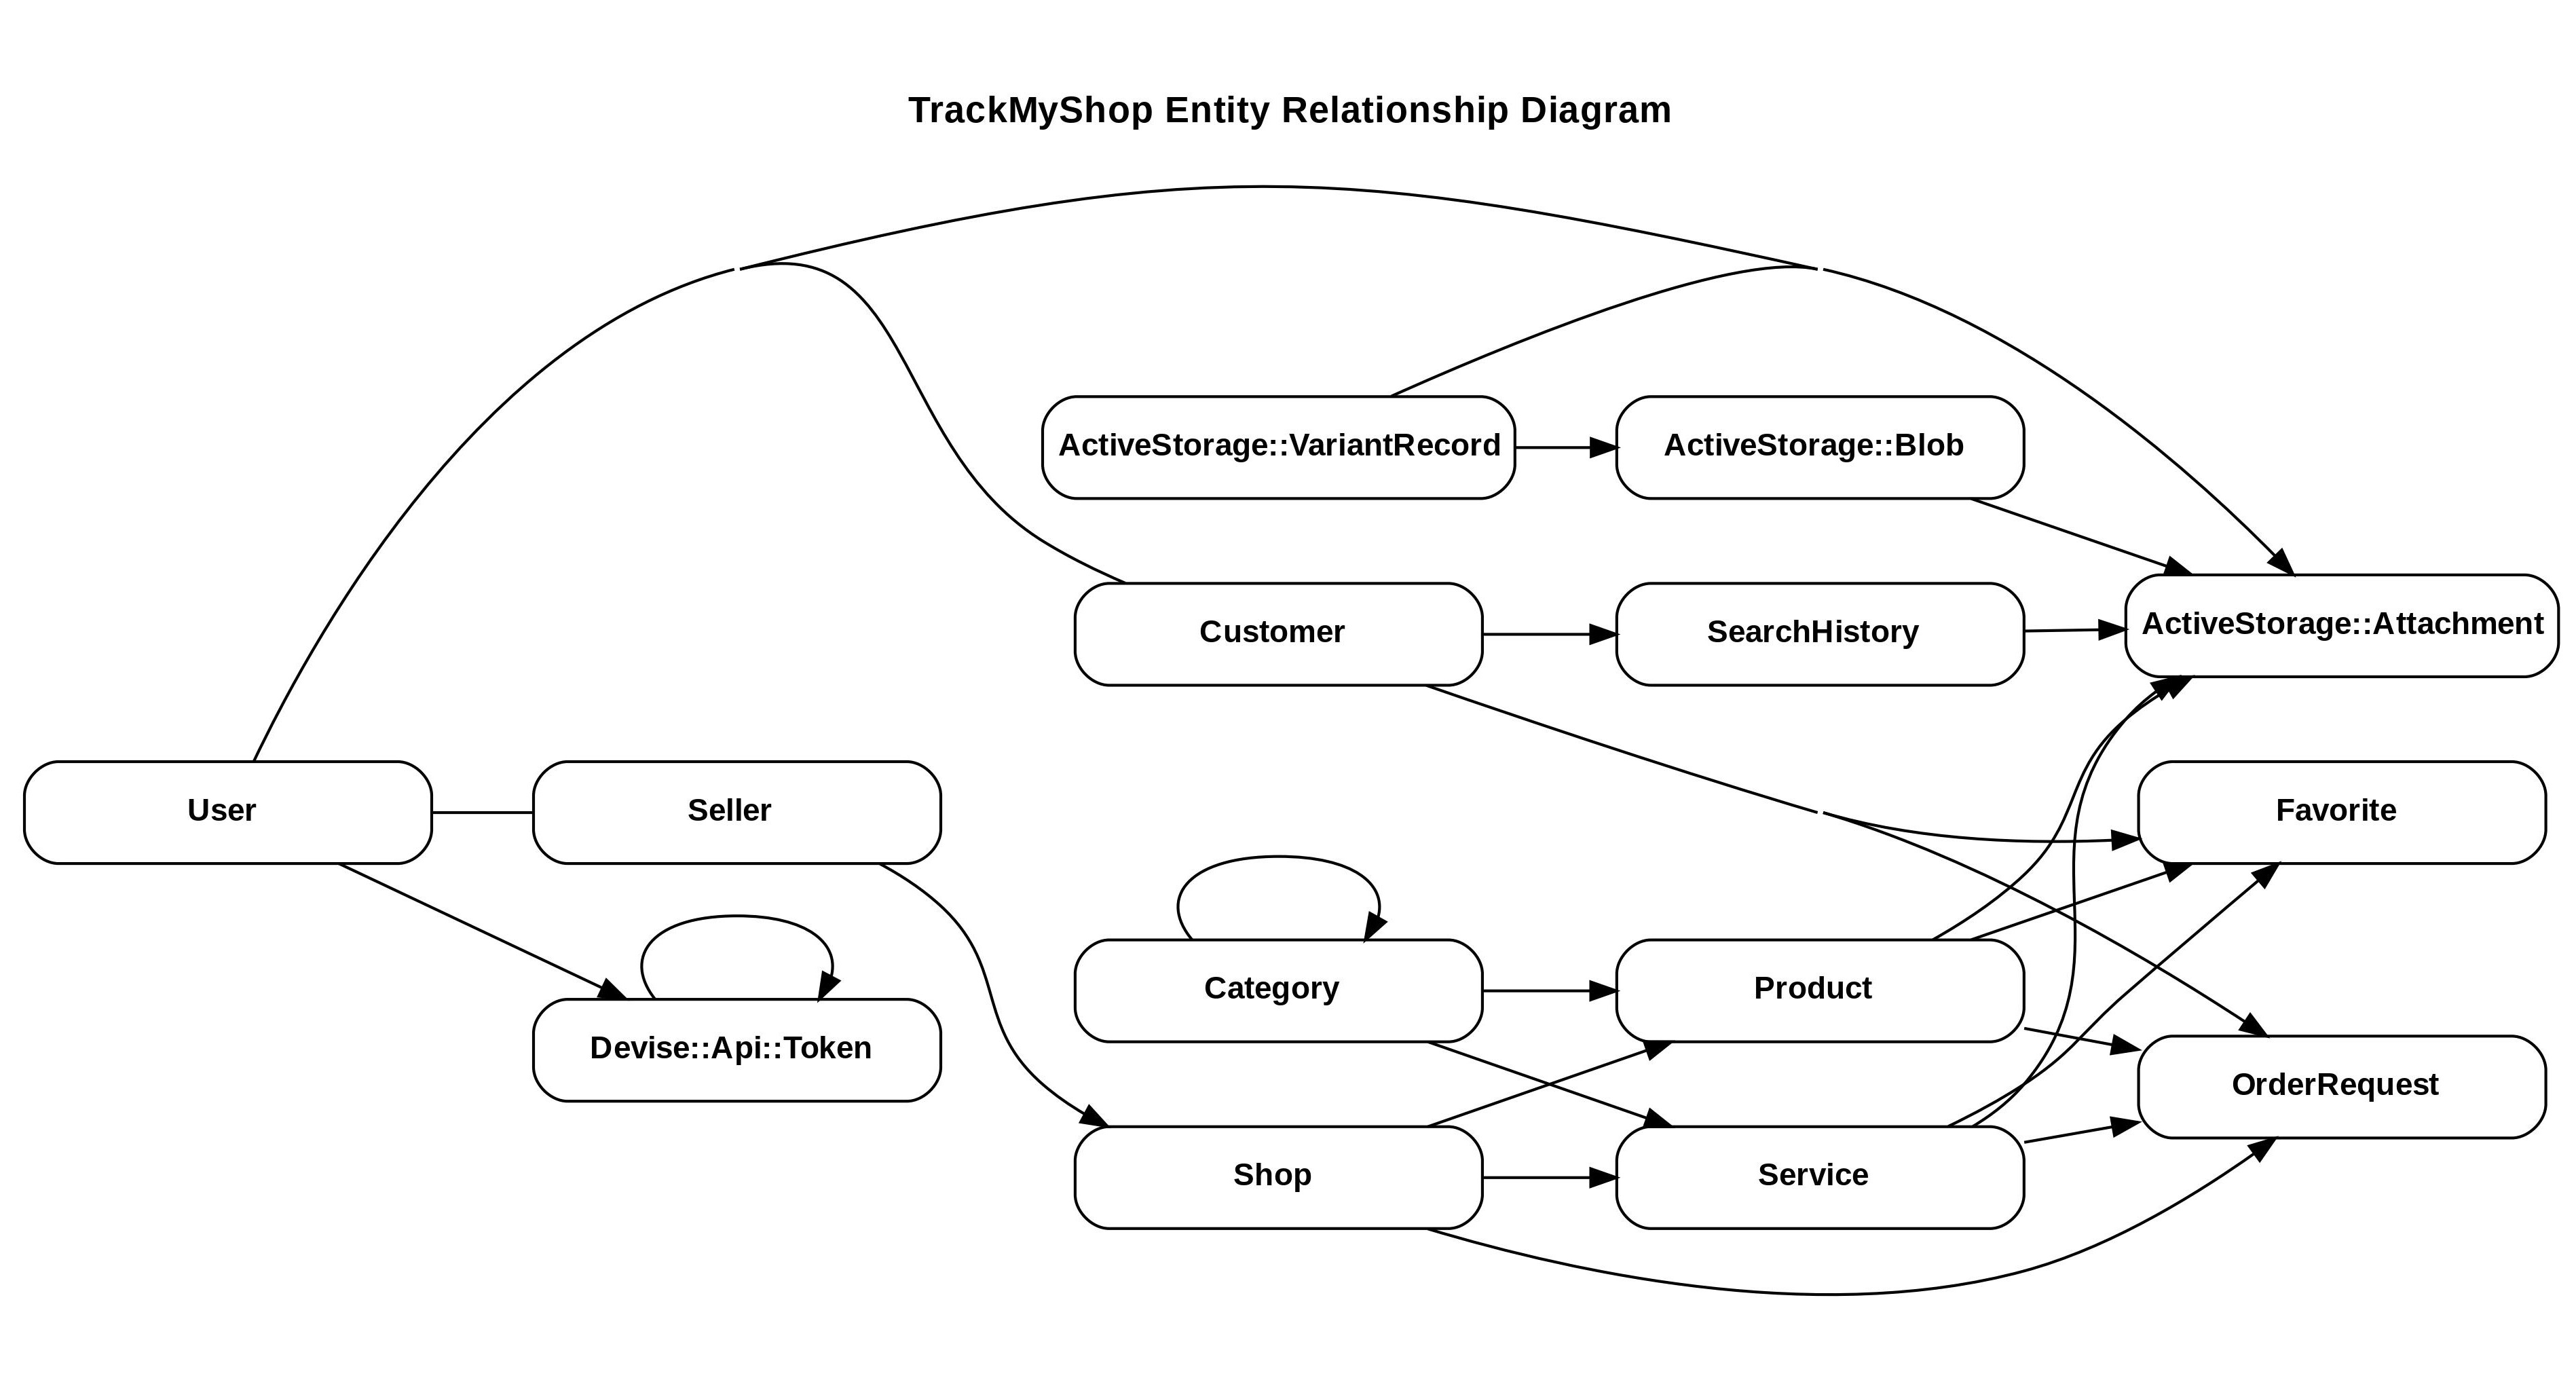
\includegraphics[width=17cm]{Entity-Relationship_Diagram}
	\caption{Track My Shop - Entity Relationship Diagram}
\end{figure}


\begin{figure}[h]
	\subsection{Class Diagram (UML) }
	\centering
	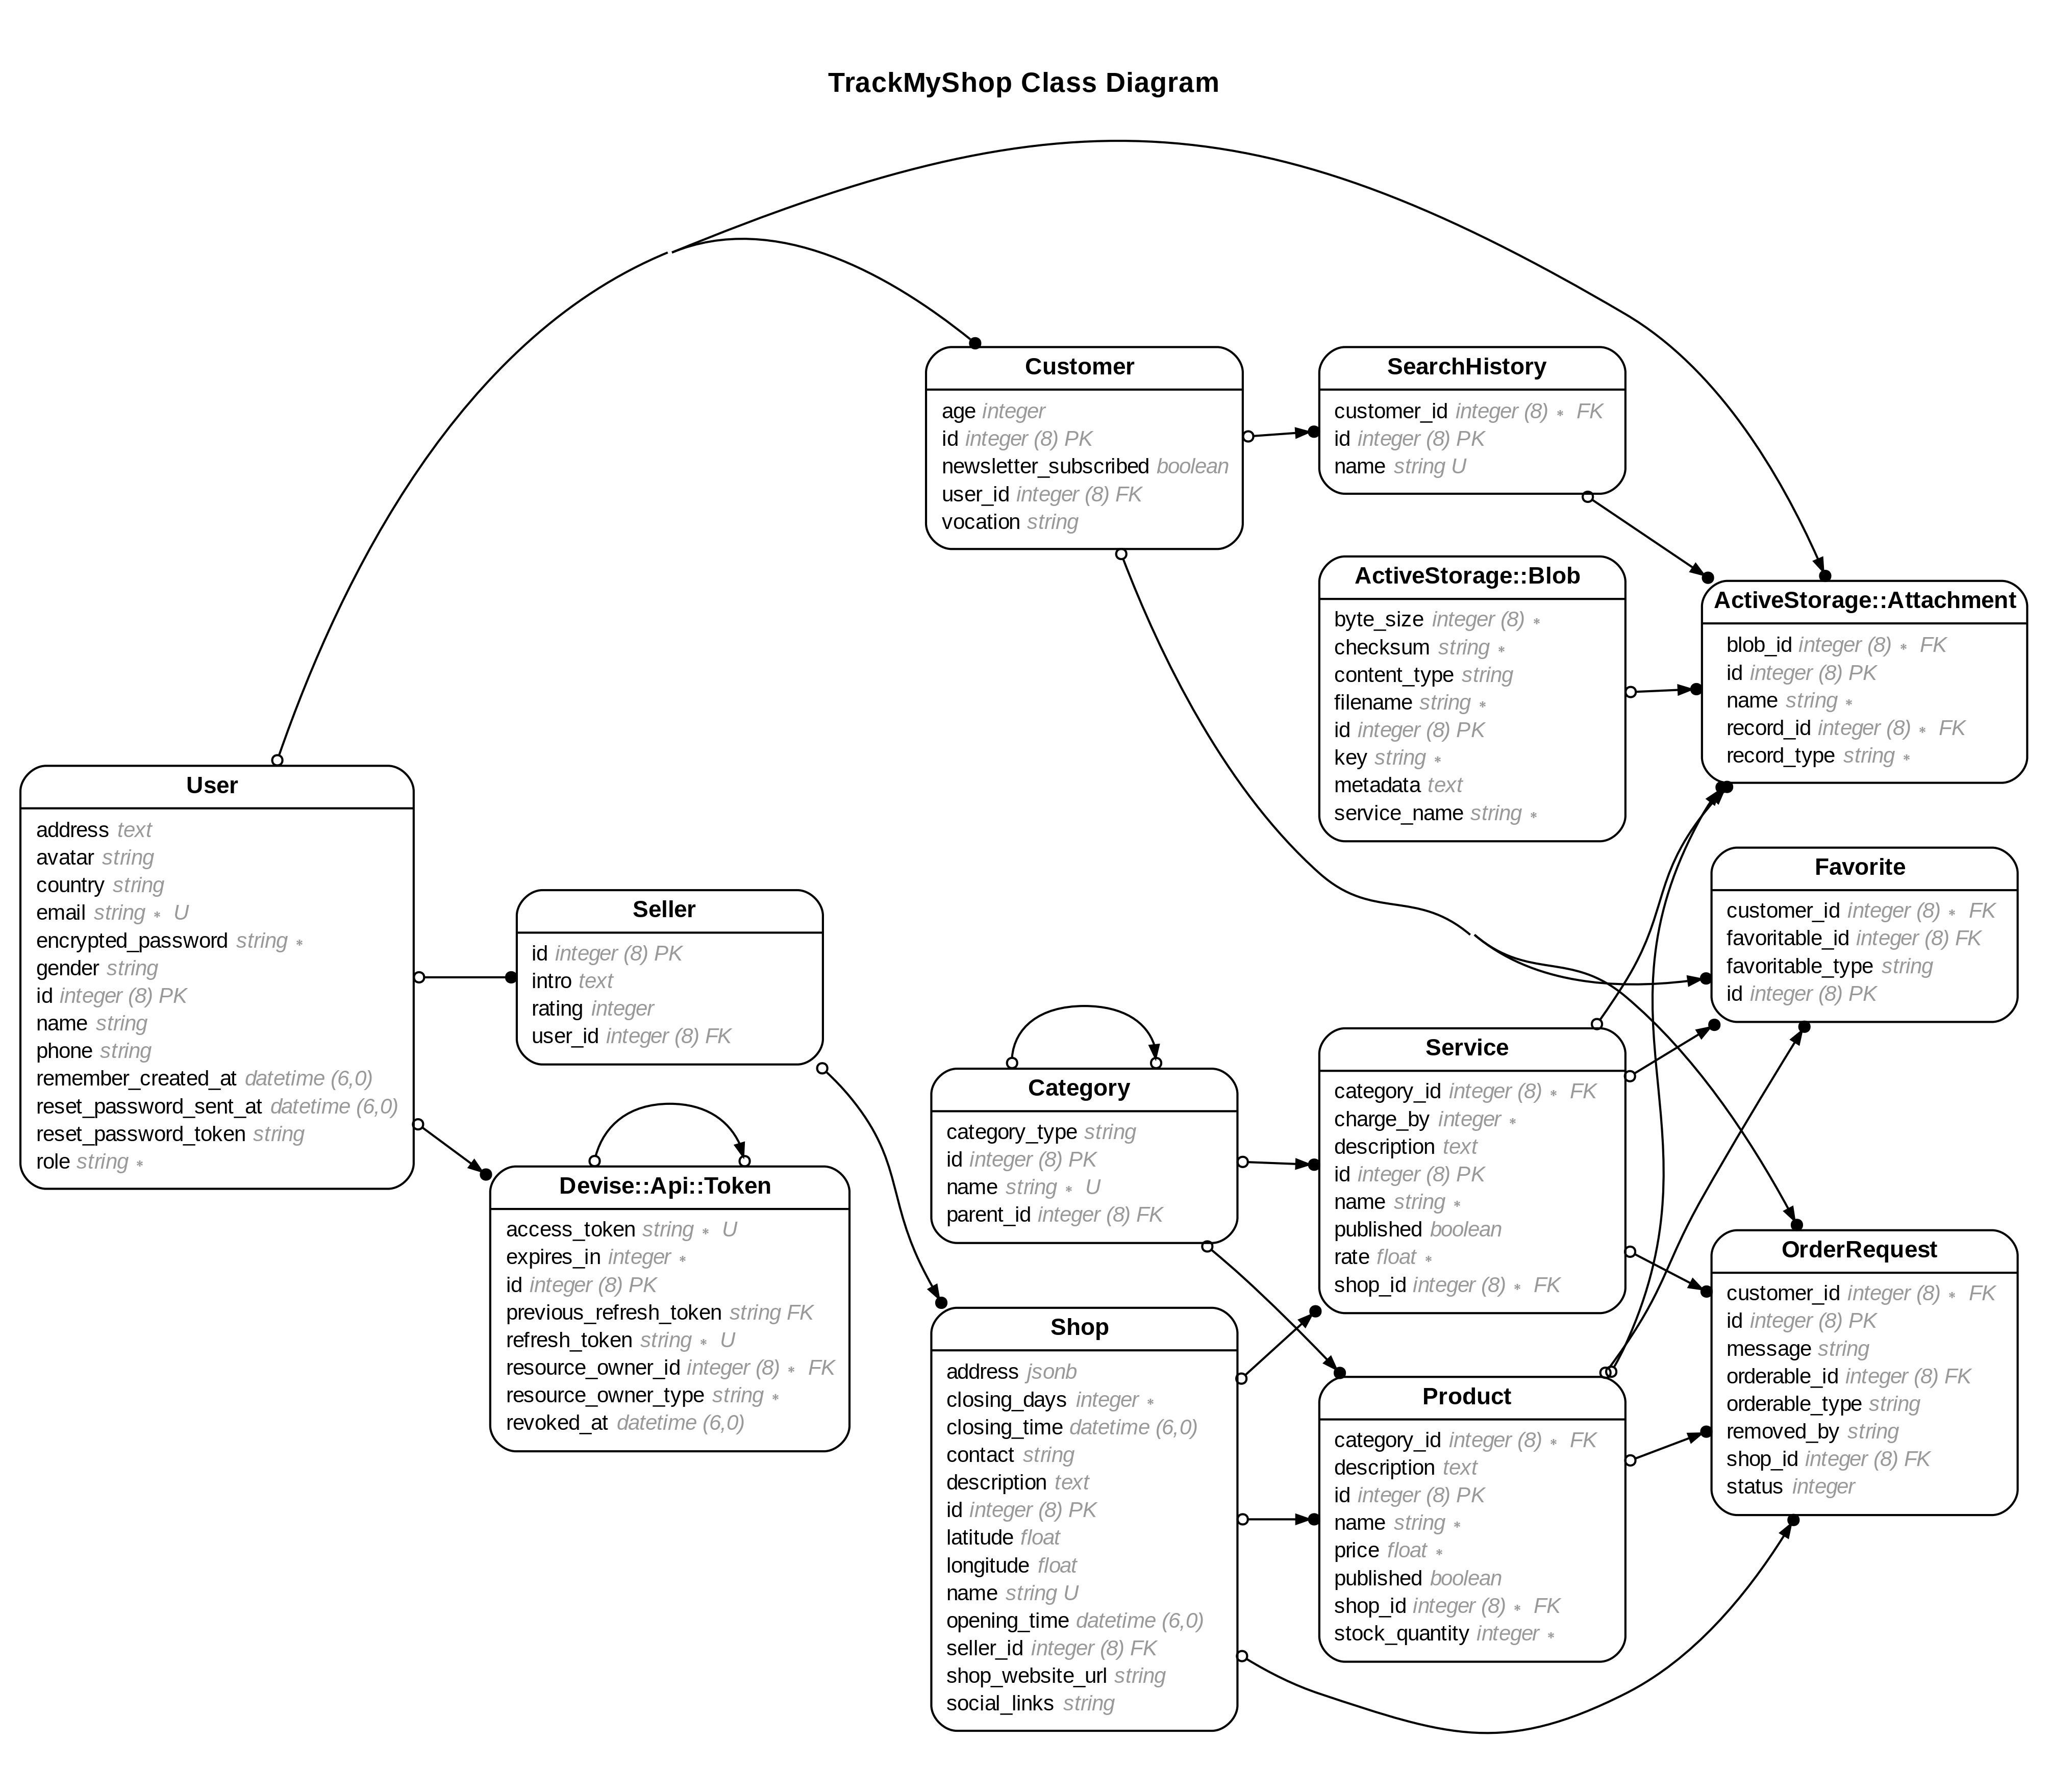
\includegraphics[width=17cm]{TrackMyShop_CD}
	\caption{Track My Shop - Class Diagram}
\end{figure}



\begin{figure}[h]
	\section{Design Description}
	Here is the basic architectural design of the Web Application:\\
	\centering
	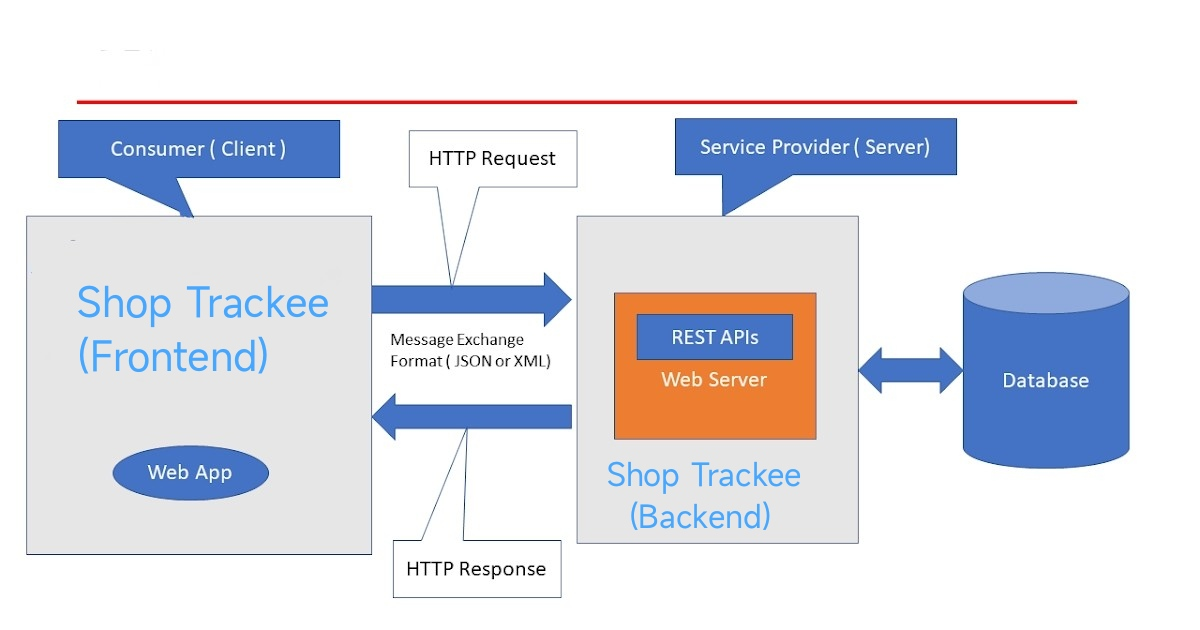
\includegraphics[width=1\linewidth]{design-description}
	\caption{Track My Shop - Design Description}
\end{figure}



